\documentclass[openany,11pt,papersize,dvipdfm]{jsbook}
\usepackage[final]{funpro}
\usepackage{graphicx}

\def\hissu{\bgroup\color{red}}
\def\endhissu{\egroup}

\thisYear{2023}

% プロジェクト名
\jProjectName{使ってもらって学ぶフィールド指向システムデザイン 2023}
\eProjectName{Field Oriented System Design Learning by Users' Feedback 2023}

% <プロジェクト番号>-<グループ名>
\ProjectNumber{3-A}

% グループ名
\jGroupName{グループ~A}
\eGroupName{Group~A}

% プロジェクトリーダ
\ProjectLeader{佐々木虎太郎}{Kotaro~Sasaki}

% グループリーダ
\GroupLeader  {及川寛太}{Kanta~Oikawa}

% メンバー数
\SumOfMembers{4}
% グループメンバ
\GroupMember {1}{及川寛太}{Kanta~Oikawa}
\GroupMember {2}{下村蒔里萌}{Marimo~Shimomura}
\GroupMember {3}{大津武琉}{Takeru~Otsu}
\GroupMember {4}{稲田敬介}{Keisuke~Inada}

% 指導教員
\jadvisor{伊藤恵,南部美砂子,奥野拓,元木環,石尾隆}
\eadvisor{Kei~Ito,Misako~Nambu,Taku~Okuno,Tamaki~Motoki,Takashi~Ishio}

% 論文提出日
\jdate{2024年1月17日}
\edate{January~17, 2024}

\begin{document}
%
% 表紙
\maketitle

%======================================================================
%前付け
\frontmatter

% 和文概要
\begin{jabstract} 日本語の概要を書く。
% 和文キーワード
\begin{jkeyword}
キーワード1, キーワード2, キーワード3, キーワード4, キーワード5
\end{jkeyword}
\bunseki{未来太郎}
\end{jabstract}

%英語の概要
\begin{eabstract} Abstract in English. 
% 英文キーワード
\begin{ekeyword}
Keyrods1, Keyword2, Keyword3, Keyword4, Keyword5
\end{ekeyword}
\bunseki{函館花子}
\end{eabstract}

\tableofcontents% 目次

%======================================================================
\mainmatter% 本文のはじまり

\chapter{背景}
%該当分野の従来の状況、問題点、本プロジェクトで設定した課題、実施した解決策、及び成果を簡潔に記述する。

\bunseki{北海花子}

\section{\midorfin{該当分野の現状と従来例}{前年度の成果}}
%プロジェクトの分野の状況や、類似プロジェクトがあればその状況を記述する。前年度からの継続課題ならば、前年度の内容も記述する。 

一般にカレーという料理は家庭でよく作られる。これまで多くの人が
おいしいカレーの作り方について試行錯誤してきている。函館の特産
品を用いた一般料理が少ない。前年度は、省略。
\bunseki{北海太郎}

\section{現状における問題点}
%現状のままでは存在する問題点について、記述する。いわば当プロジェクトの存在意義
作るたびにカレーの味が変わる。いつもおいしいものができるとは限らない。
\bunseki{未来花子}

\section{課題の概要}\label{sec:gaiyou}
% 上述の問題点を解決すべく当プロジェクトの掲げる課題の概要を述べる。
地域の特色を生かしたおいしいカレーの作り方が課題。

\bunseki{未来太郎}
% 背景
\chapter{プロダクト}

\section{アプリケーションのコンセプト}
BuLoは,バスに乗り遅れたくないがバスを効率的に使いたいひとのためのバスロケーションアプリである.
従来のバスロケーションアプリやGoogle Mapsなどの地図アプリとは異なり,バスの位置や遅延情報をリアルタイムにわかりやすく把握することができる.
また,本サービスは``ひとめぼれ''するバスロケーションアプリをめざしている.我々は``ひとめぼれ''を以下の2つと考える.
まず1つ目にアプリのデザインに対する``ひとめぼれ''である.これは本サービスを使うきっかけとなるものである.
2つ目にアプリ全体を通しての体験への``ひとめぼれ''である.これは本サービスを使い続けるきっかけになると考える.
\bunseki{下村蒔里萌}

\section{機能}
\subsection{住所を登録}
本サービスは自宅と職場の住所を登録する機能を搭載している.
対象ユーザは通勤・通学にバスを利用する人であり,使用するルートは変わらないことが予測できるため,最初に住所を登録をすることで2回目以降は再度住所の検索をする手間を省いている.
図\ref{fig:feature_register}の左から3枚目の画面では,現在地の住所をサジェストしている.
住所の入力では,キーワードに対しての予測をサジェストしている.
\begin{figure}
    \centering
    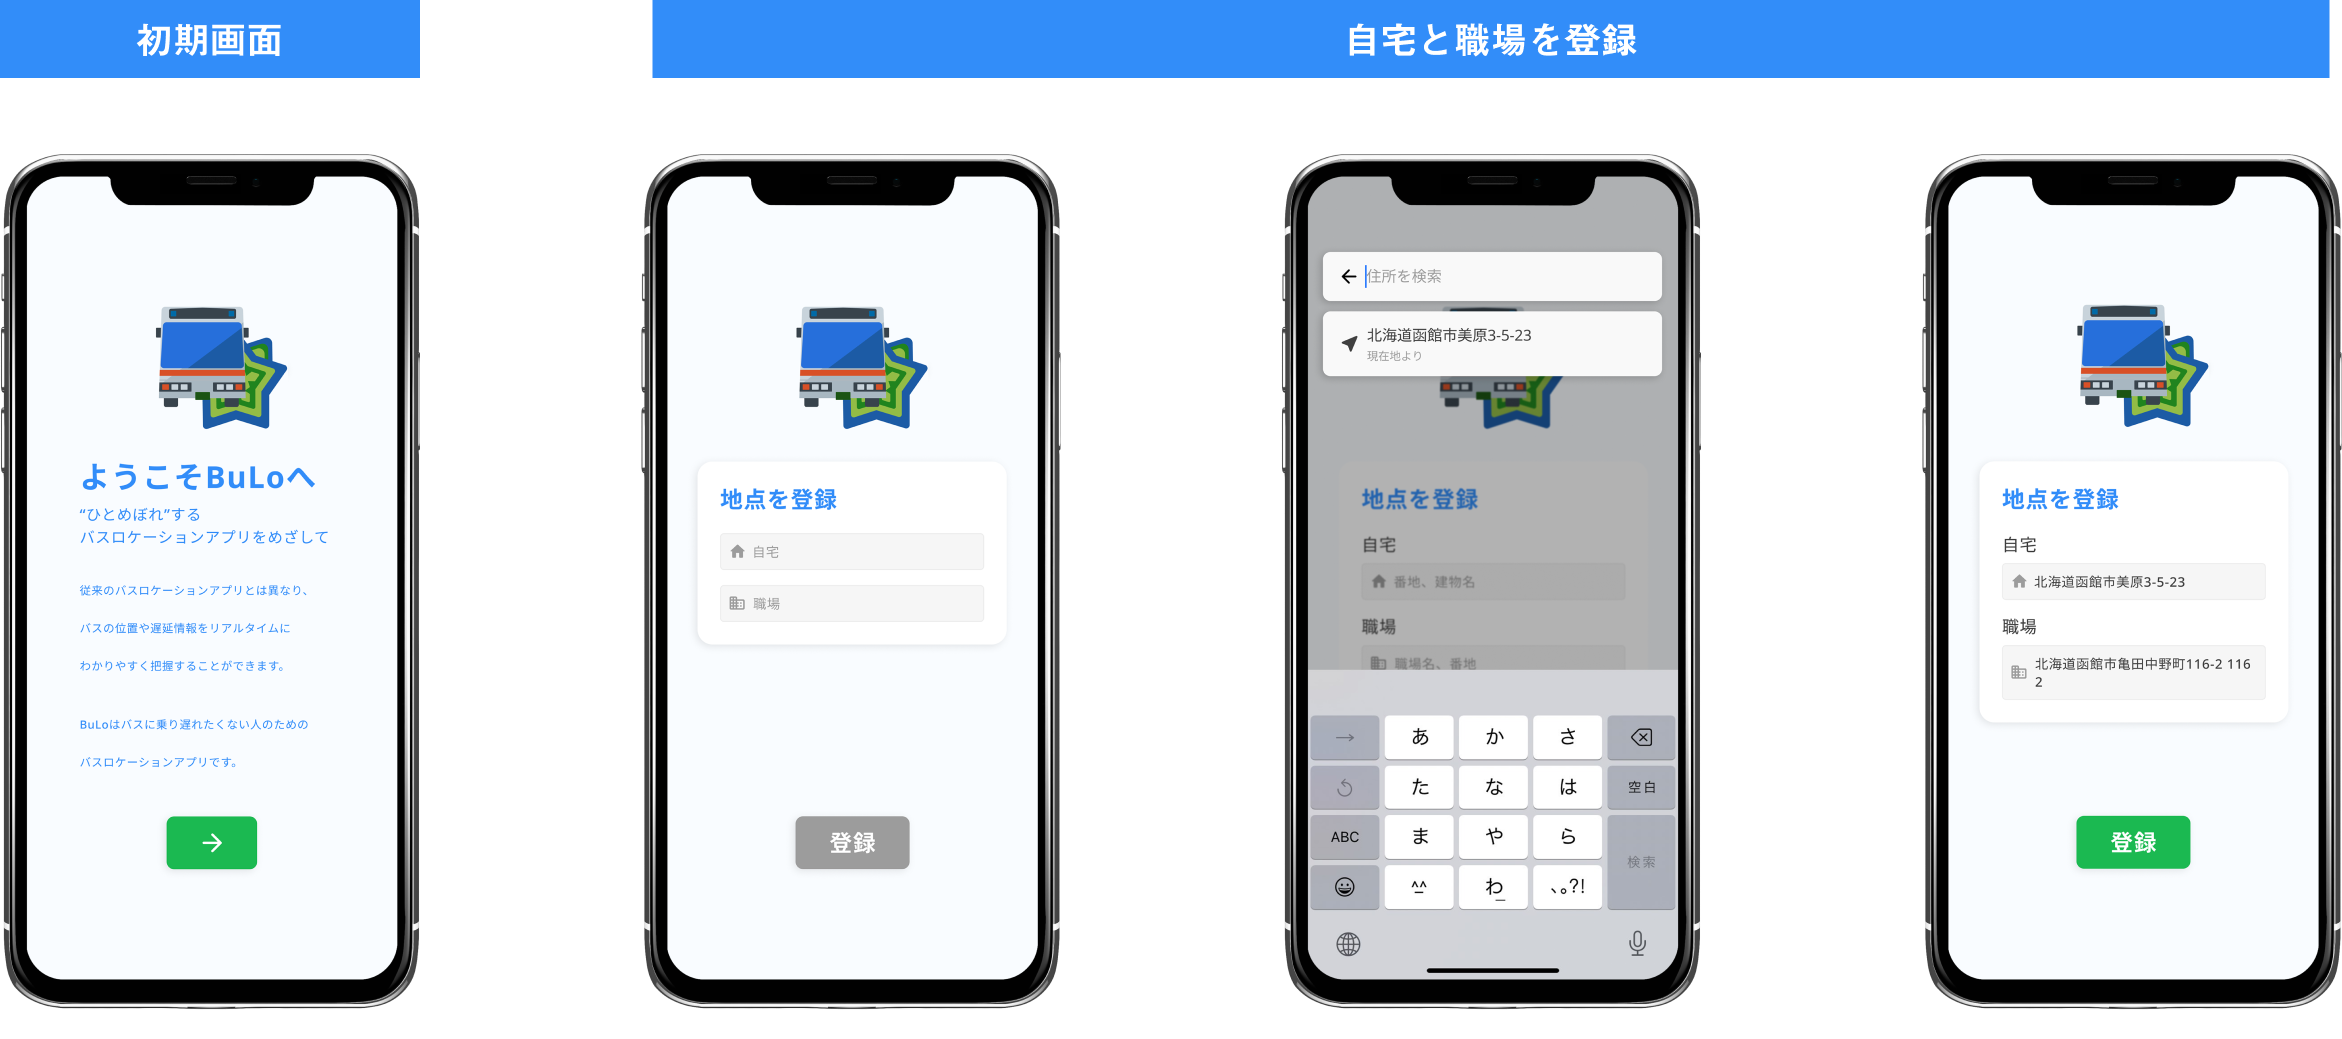
\includegraphics[width=14cm]{images/feature_register.png}
    \caption{住所を登録}
    \label{fig:feature_register}
\end{figure}
\subsection{Time-Distance ListとRoute View}
ユーザが住所を登録したあと,ユーザがアプリを開いた際は図\ref{fig:feature_td}の画面を表示する.
図\ref{fig:feature_td}の左側の画面は,後述するTime-Distance Viewの一覧である.
一覧は,バスがユーザの乗車するバス停に到着する順に表示される.
図\ref{fig:feature_td}の右側の画面は,各Time-Distance Viewをタップした際に表示される画面である.
ここではタップしたTime-Distance Viewと,ユーザとそのバスの現在地がマップ上に表示される.
\begin{figure}
    \centering
    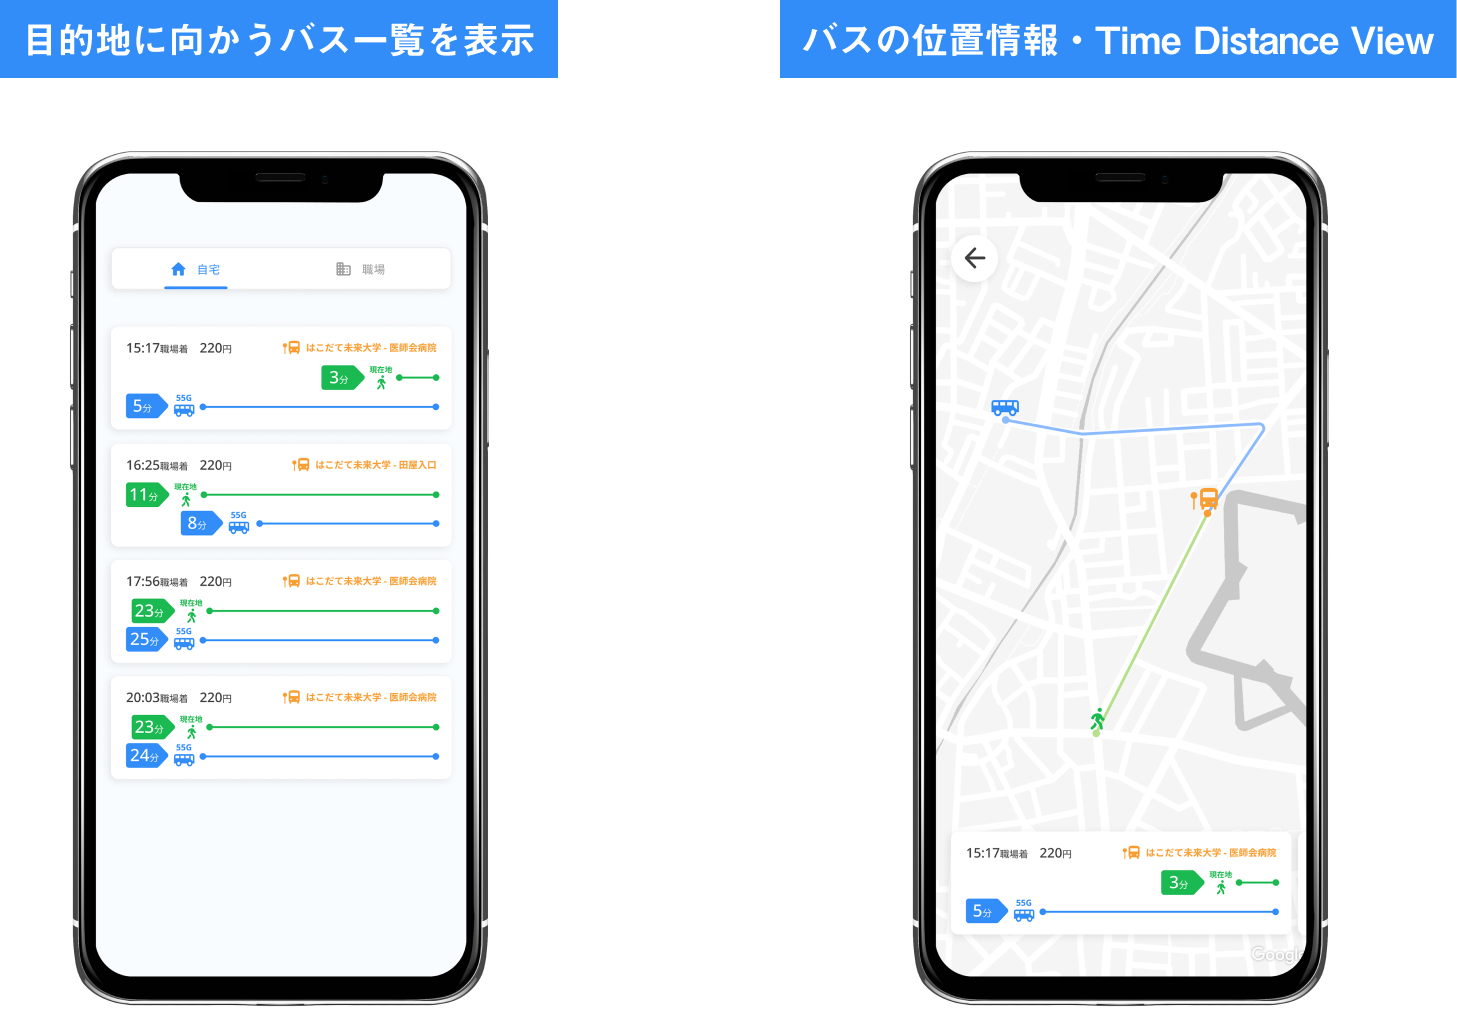
\includegraphics[width=14cm]{images/feature_td.png}
    \caption{Time-Distance ViewとRoute View}
    \label{fig:feature_td}
\end{figure}
\subsection{Time-Distance Viewの詳細}
Time-Distance Viewとは,ユーザの現在地・バスの現在地・バス停の3点を時間的グラフに表したものである.
これにより,ユーザは「バスに間に合うかどうか」,「バス停でどのくらい待つか」がひとめでわかる.
実装方法は図\ref{fig:feature_timedistanceview}に示す.
また,図\ref{fig:feature_timedistanceview}では以下の状況を考えている.
\begin{quote}
    \begin{itemize}
        \item ユーザの目的地は自宅(田屋入口の近く)
        \item 現在地からの最寄りのバス停ははこだて未来大学駅
        \item ユーザが乗るバスは55G
        \item ユーザが自宅に行くまでにかかる料金は220円
        \item バスは5分後にはこだて未来大学駅に到着する
        \item 現在地からはこだて未来大学駅まで徒歩で3分かかる
        \item 自宅には16:25に到着する
    \end{itemize}
\end{quote}
\begin{figure}
    \centering
    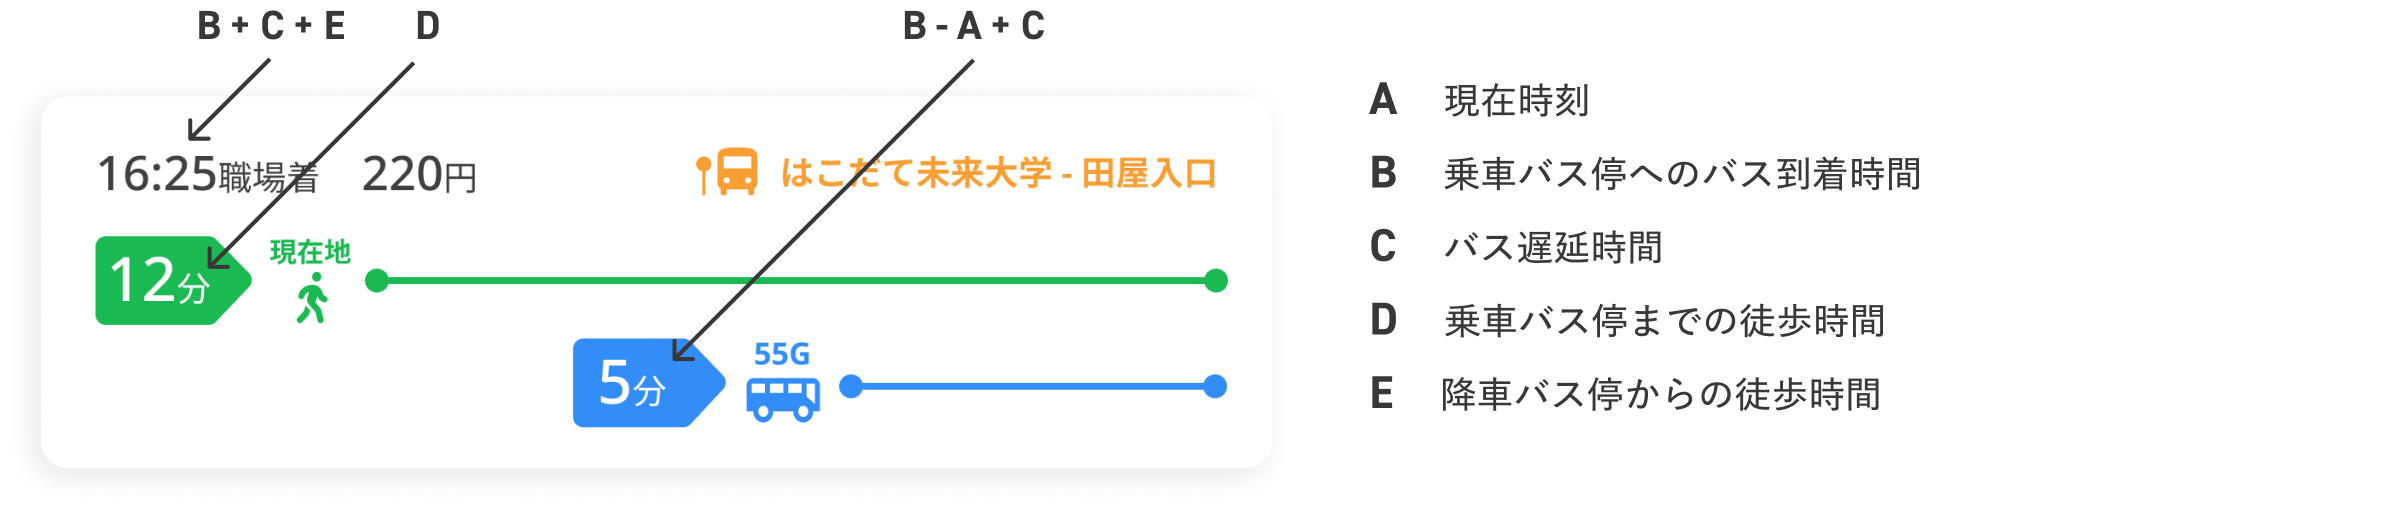
\includegraphics[width=14cm]{images/feature_timedistanceview.png}
    \caption{Time-Distance View}
    \label{fig:feature_timedistanceview}
\end{figure}
図\ref{fig:feature_timedistanceview2}では,想定されるTime-Distance Viewの例を示している.
図\ref{fig:feature_timedistanceview2}の左から,「ユーザがバスに安心して乗れる状態」
「ユーザがバス停でかなり待つことが予想できるため,バス停以外の場所で時間をつぶすことができる」
「ユーザよりバスの方が先にバス停に到着するが,走ることでバスに乗ることができる」状態である.
\begin{figure}
    \centering
    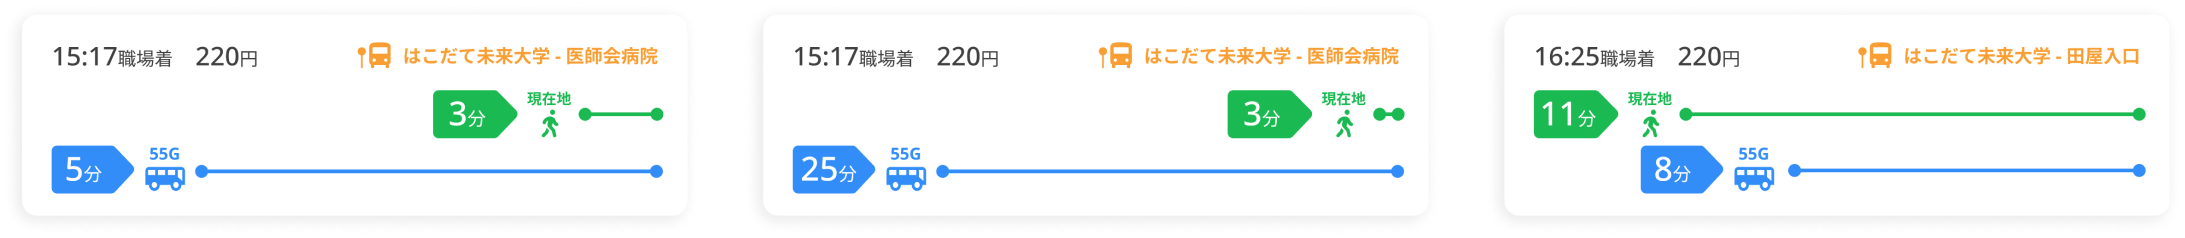
\includegraphics[width=14cm]{images/feature_timedistanceview2.png}
    \caption{Time-Distance Viewの例}
    \label{fig:feature_timedistanceview2}
\end{figure}
\bunseki{下村蒔里萌}

\section{デザインシステム}
本アプリは,簡潔で見やすく情報量の絞られたデザインを目指している.
アジャイル開発を行う上で,手戻りの少ない一貫性のあるUI改善を行うため,また,エンジニアとデザイナーの共通認識を図るために,
以下のデザインシステムを設定した.
\subsection{Colors}
本サービスのカラーパレットは図\ref{fig:feature_colors}のように設定した.
16進数のカラーコード(例:\#FF3B30)に具体的な値を与え使いやすくしたプリミティブトークン(例:red)と,
特定の用途別に定義したセマンティックトークン(例:alert)を定義している.
Figma上でのプロトタイプや実装では,セマンティックトークンを使用した.
\begin{figure}
    \centering
    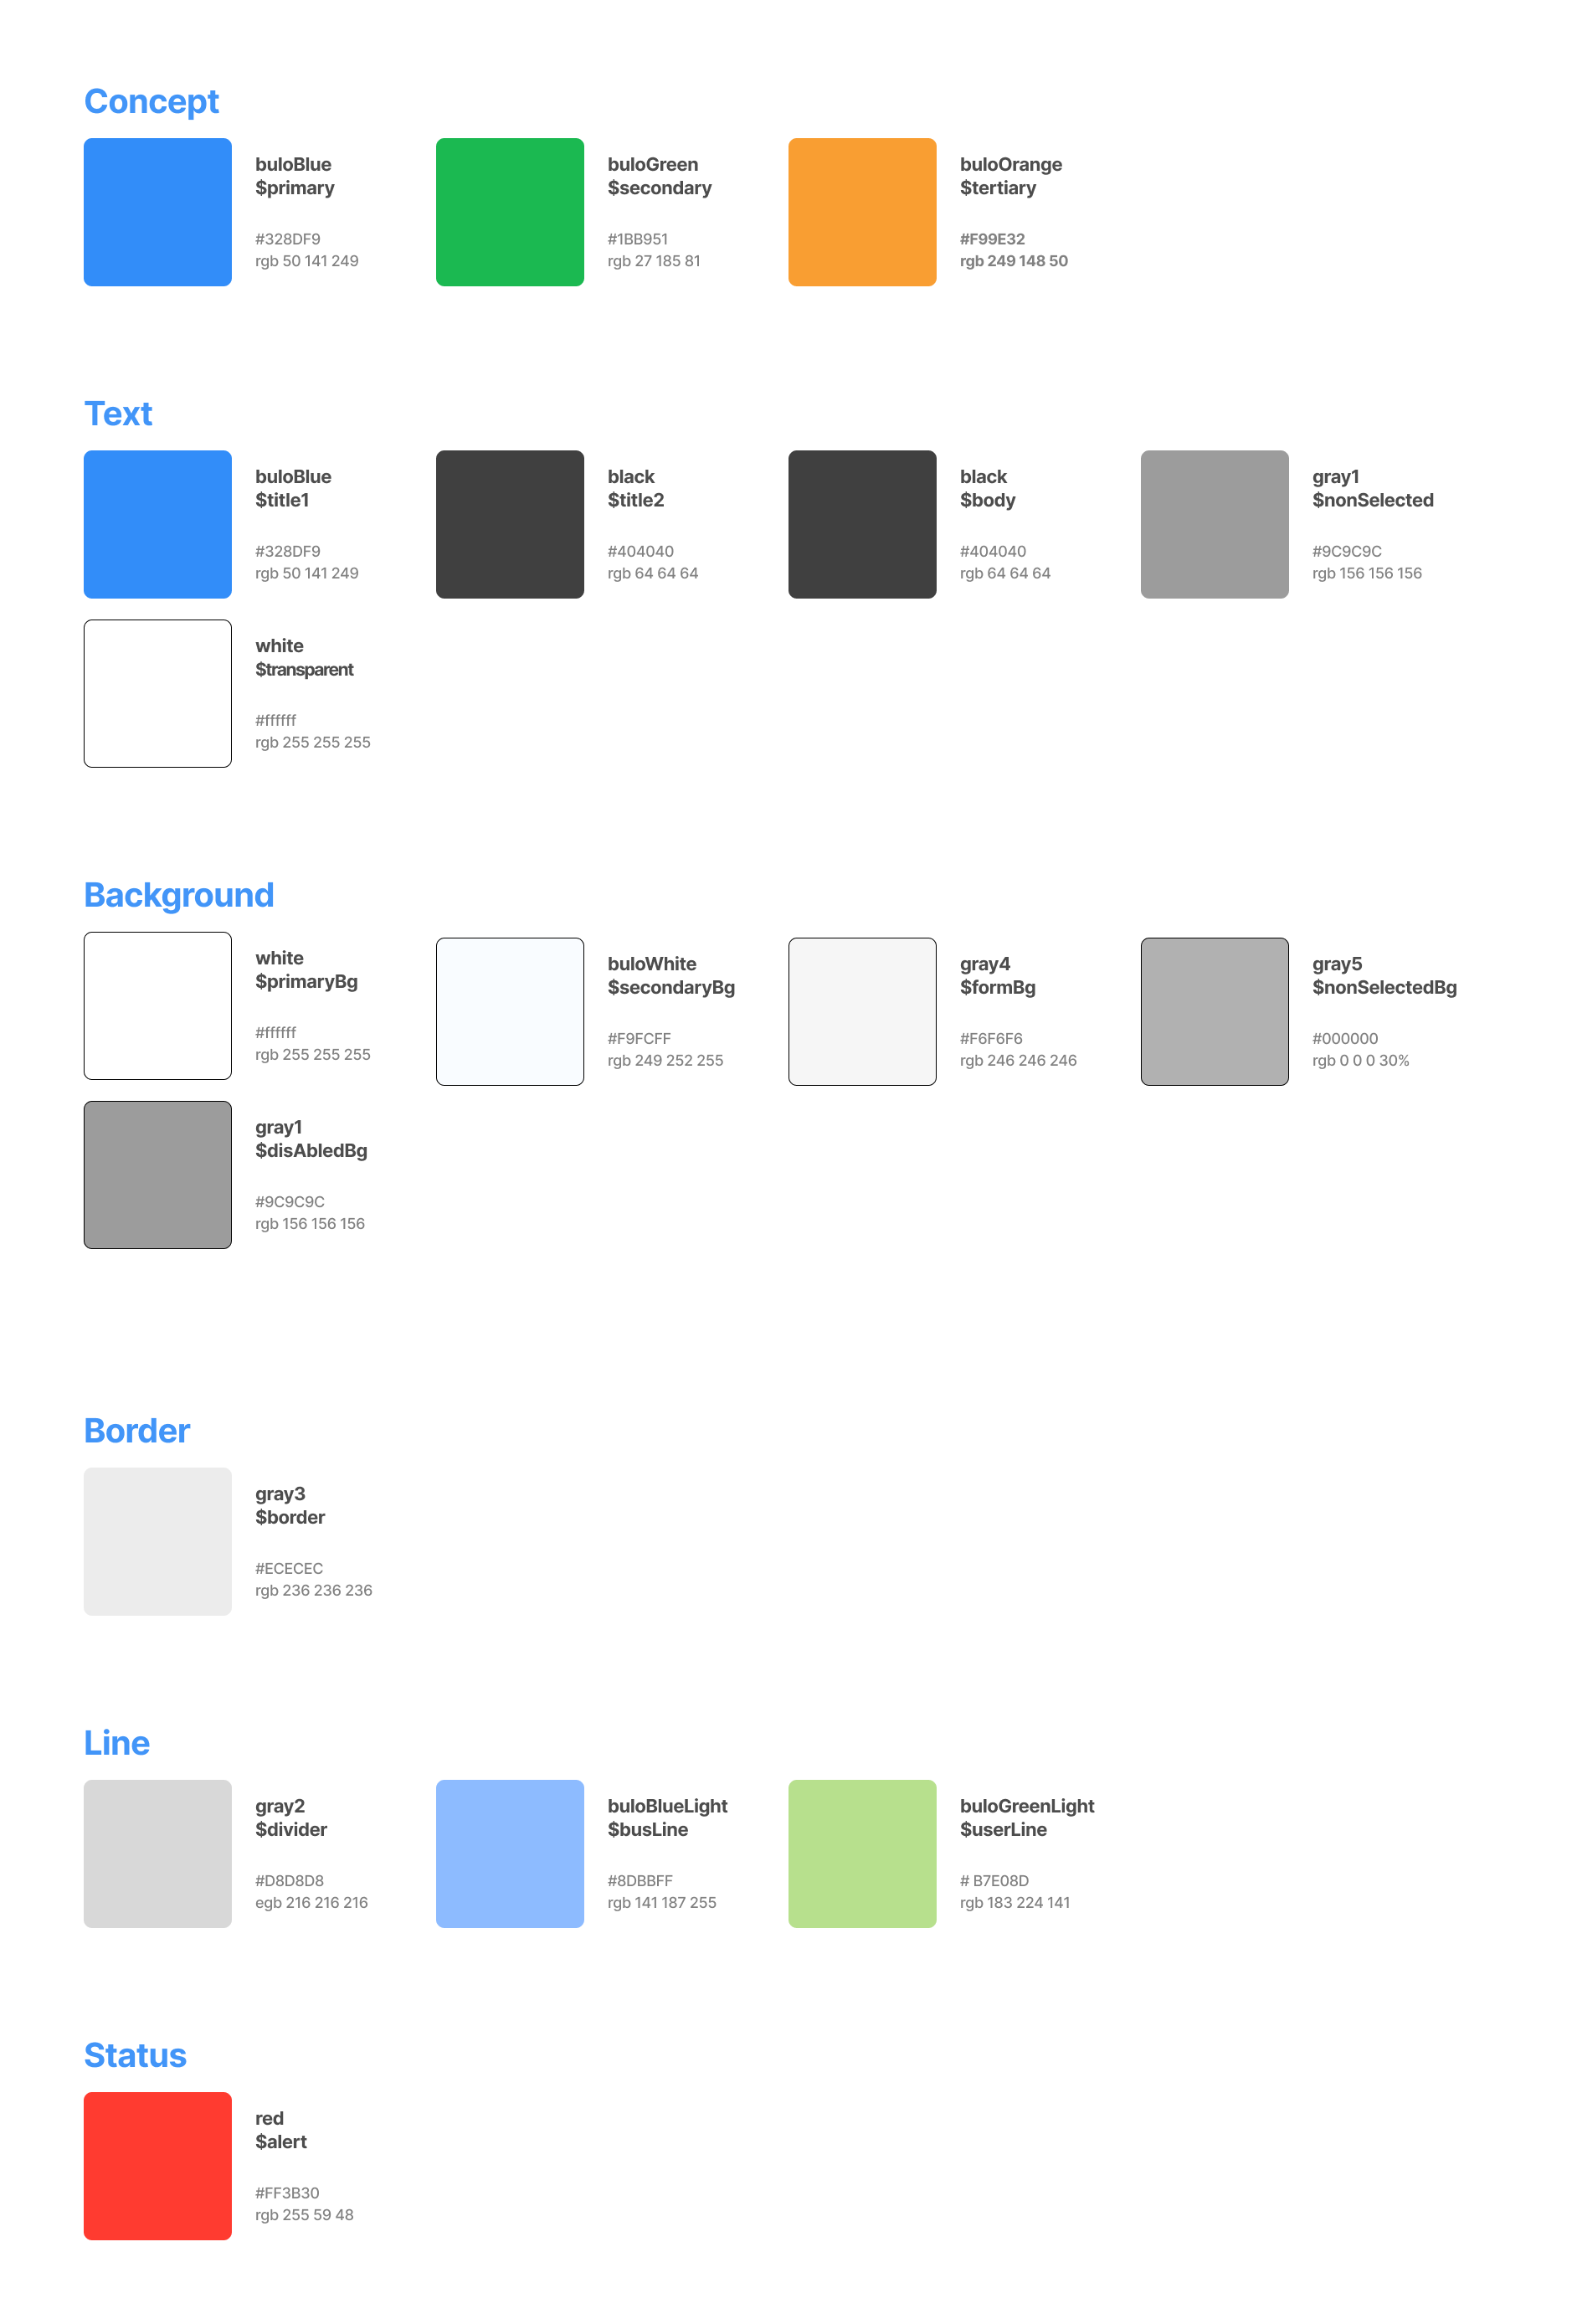
\includegraphics[width=10cm]{images/colors.png}
    \caption{デザインシステム Colors}
    \label{fig:feature_colors}
\end{figure}
\subsection{Typographies}
本サービスのフォントは図\ref{fig:typographies}のように設定した.
\begin{figure}
    \centering
    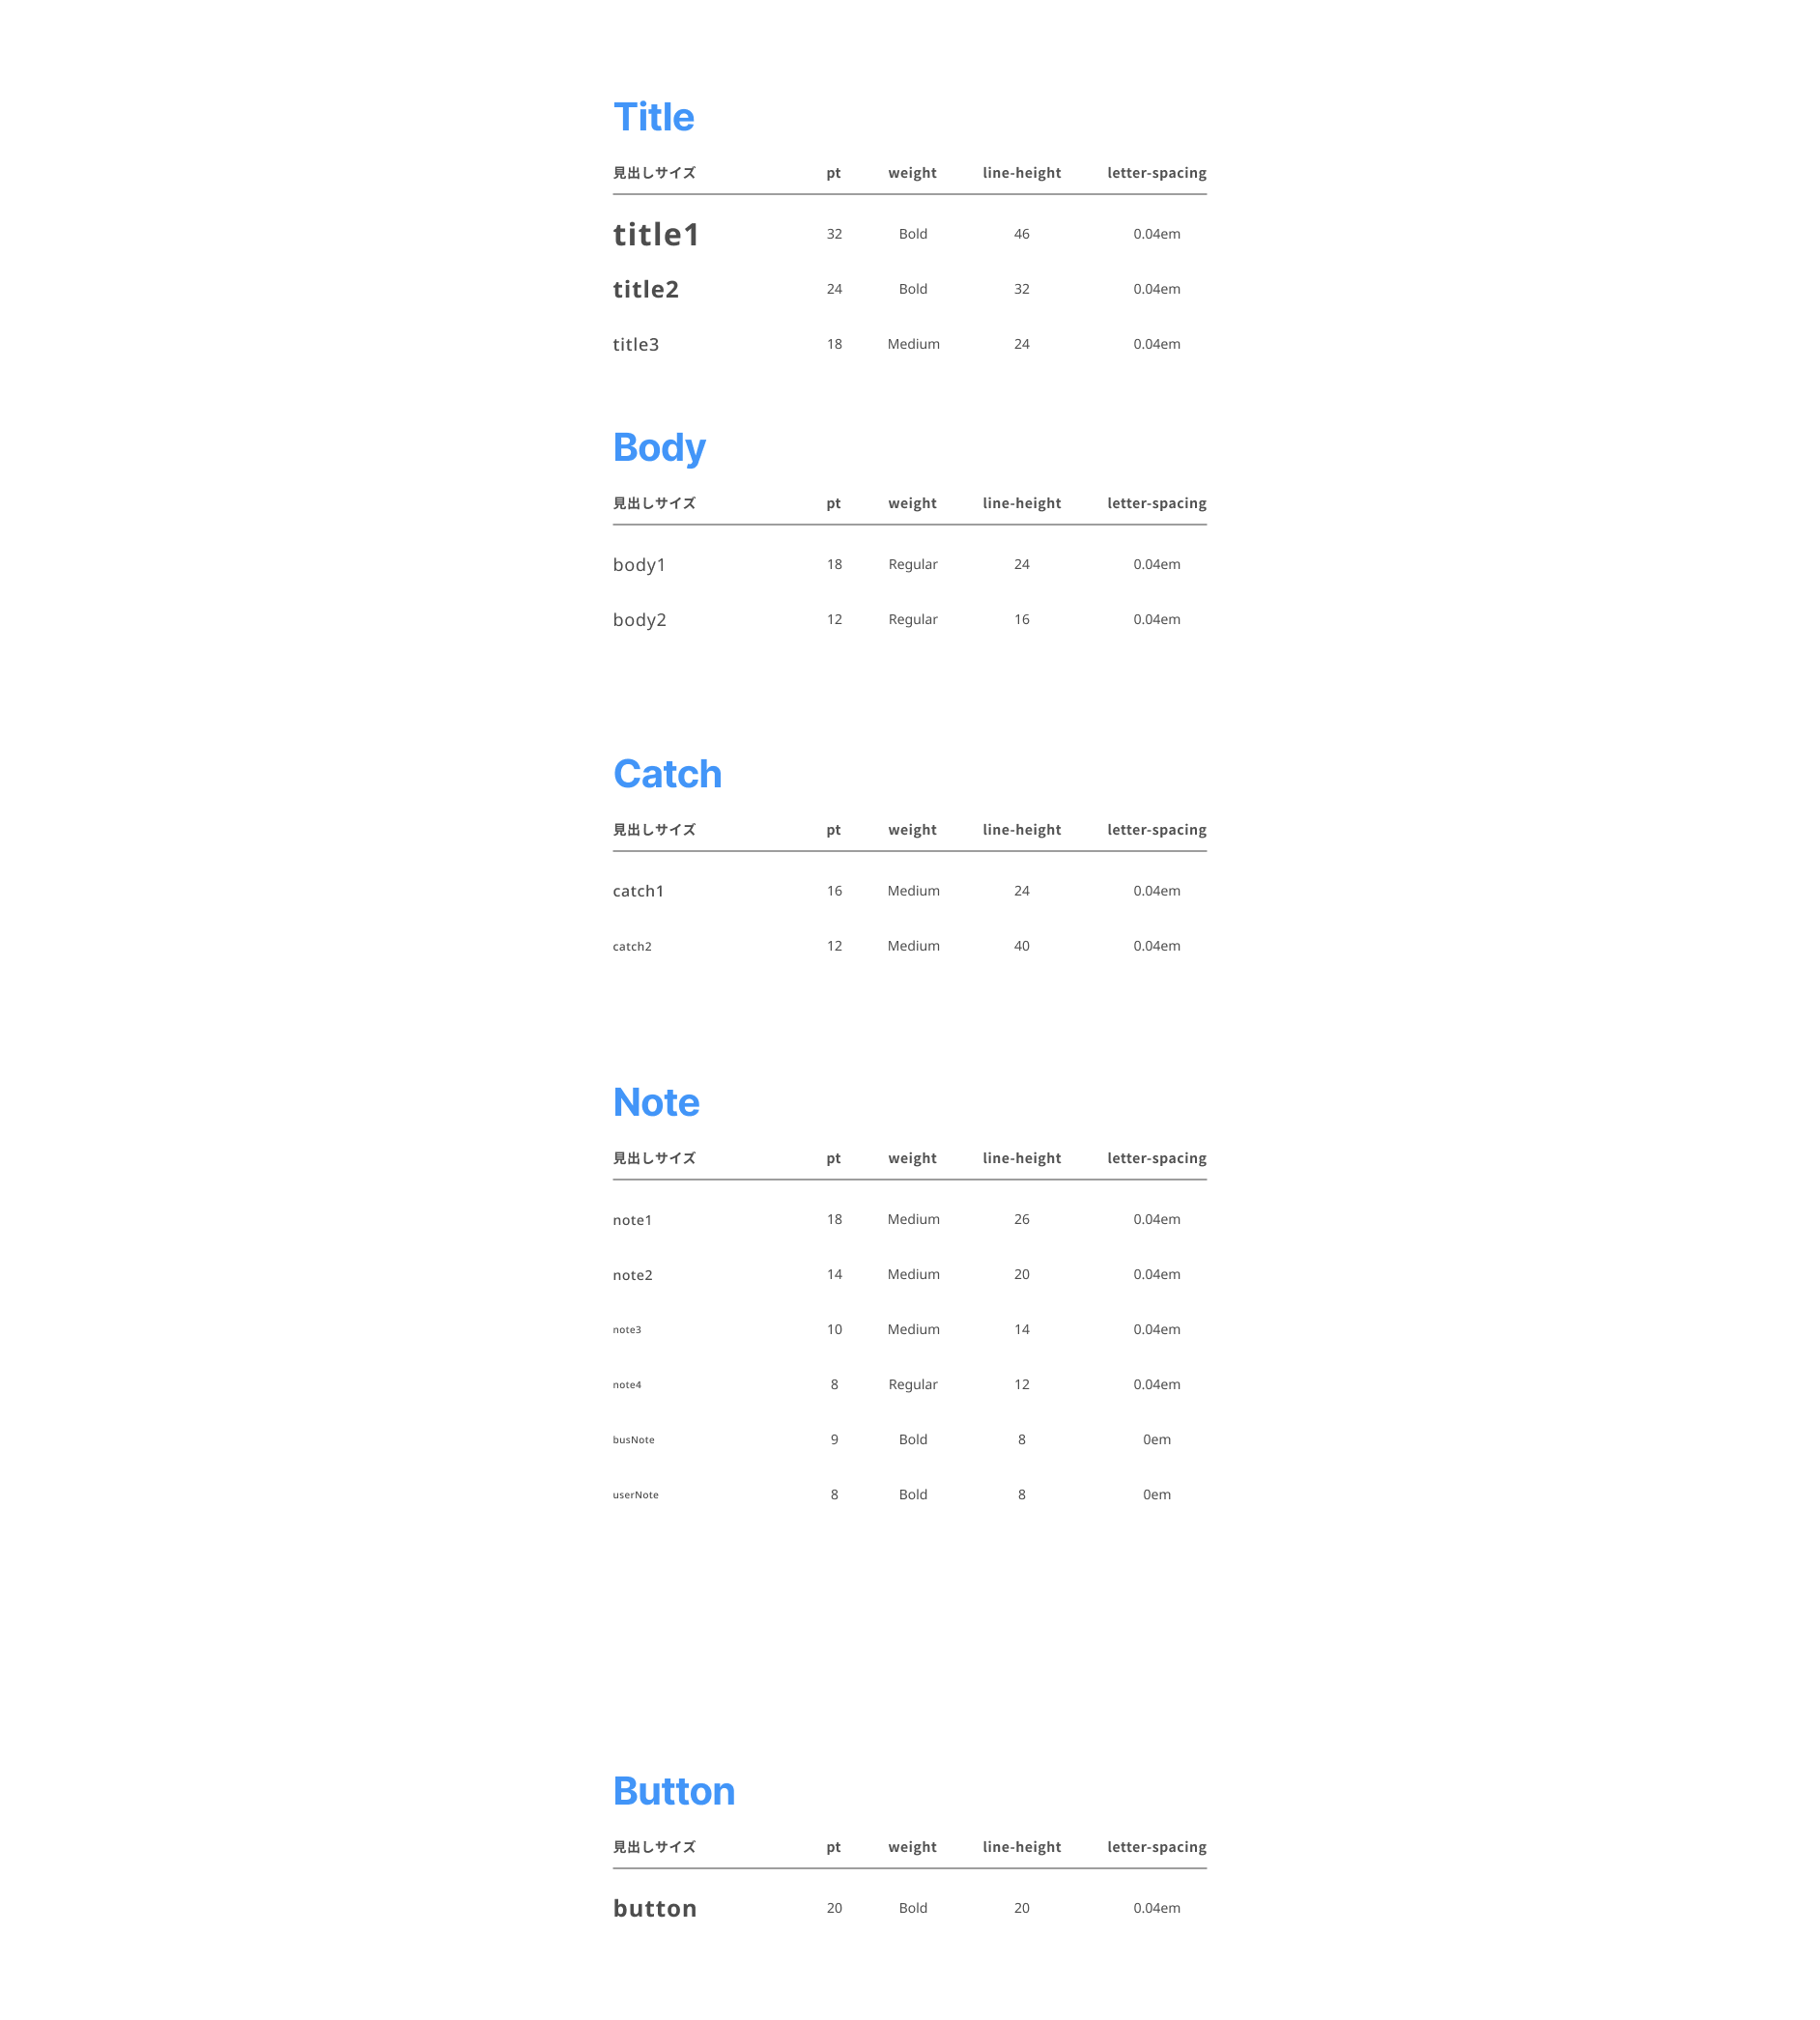
\includegraphics[width=10cm]{images/typographies.png}
    \caption{デザインシステム Typographies}
    \label{fig:typographies}
\end{figure}
\subsection{Icons}
    本サービスのアイコンは図\ref{fig:icons}のように設定した.
    主にMaterial Symbols and Icons\footnote{https://fonts.google.com/icons}を使用し,足りないものはPictogrammers\footnote{https://pictogrammers.com/}を使用した.
        \begin{figure}
            \centering
            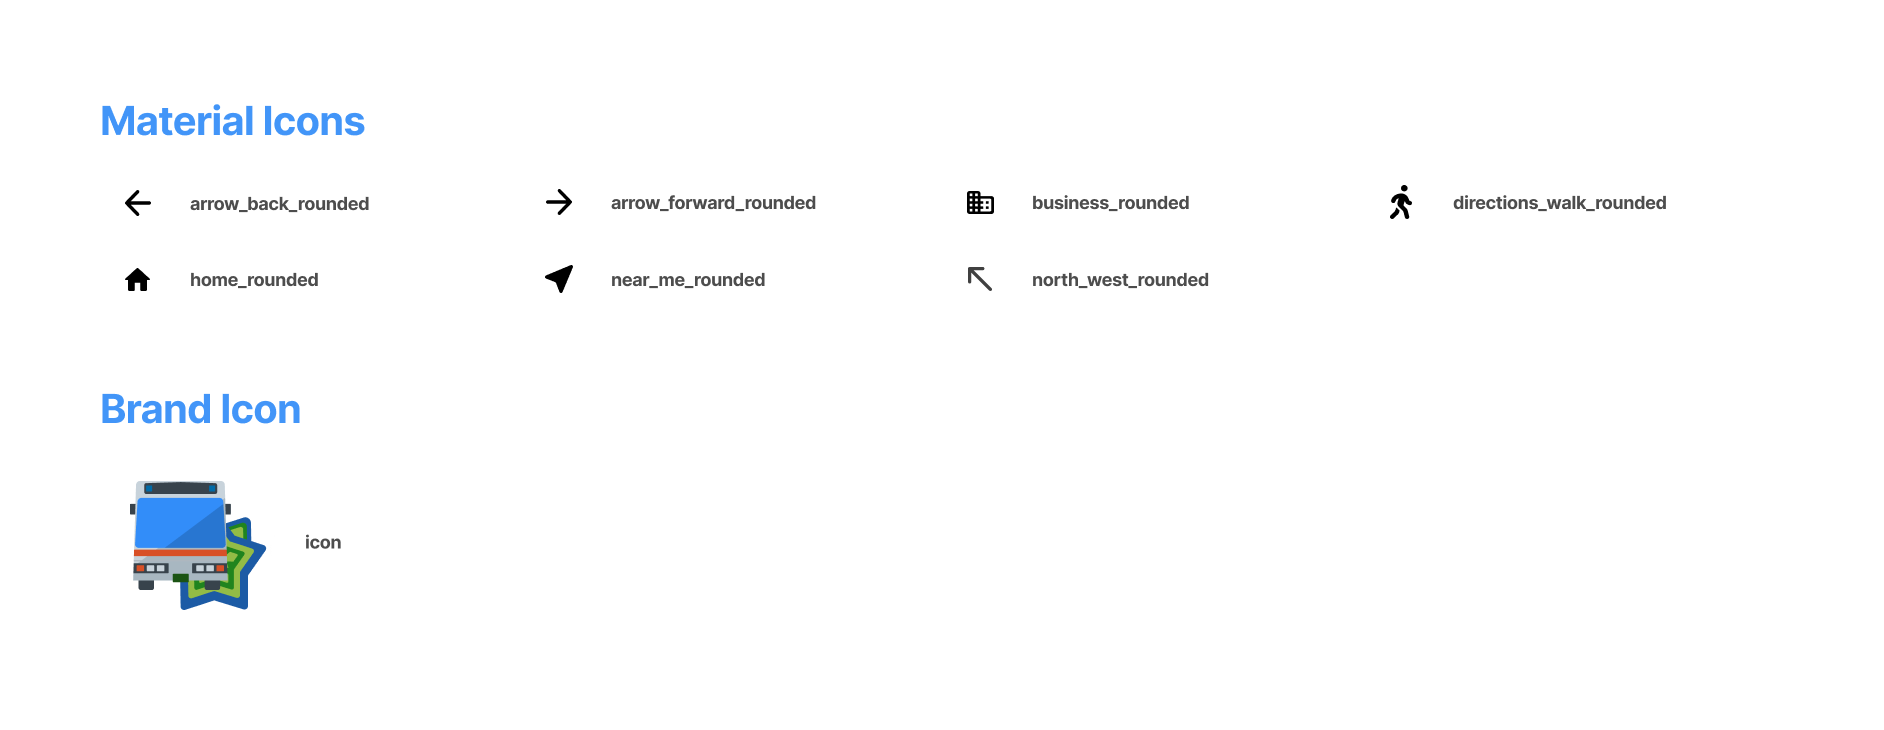
\includegraphics[width=10cm]{images/icons.png}
            \caption{デザインシステム Icons}
            \label{fig:icons}
        \end{figure}
\subsection{Shapes and Others}
    本サービスの形状とその他のデザインは図\ref{fig:shapes}のように設定した.
    ElevationやBlurは2つのレイヤー間のz軸上の深度を表す.
    インターフェイス上の最も上位の要素をより強調することで,アクションの重要度を伝える.
    Cornersは角丸を表し,4, 8, 16と3種類の数字を用意し,コンポーネントの短辺に合わせて角丸の数値を可変する.
    角丸を使用した図形の中に,角丸を使用した図形位がある場合は,
    外側の図形の角丸=内側の図形の角丸+内側の余白とする.
\begin{figure}
    \centering
    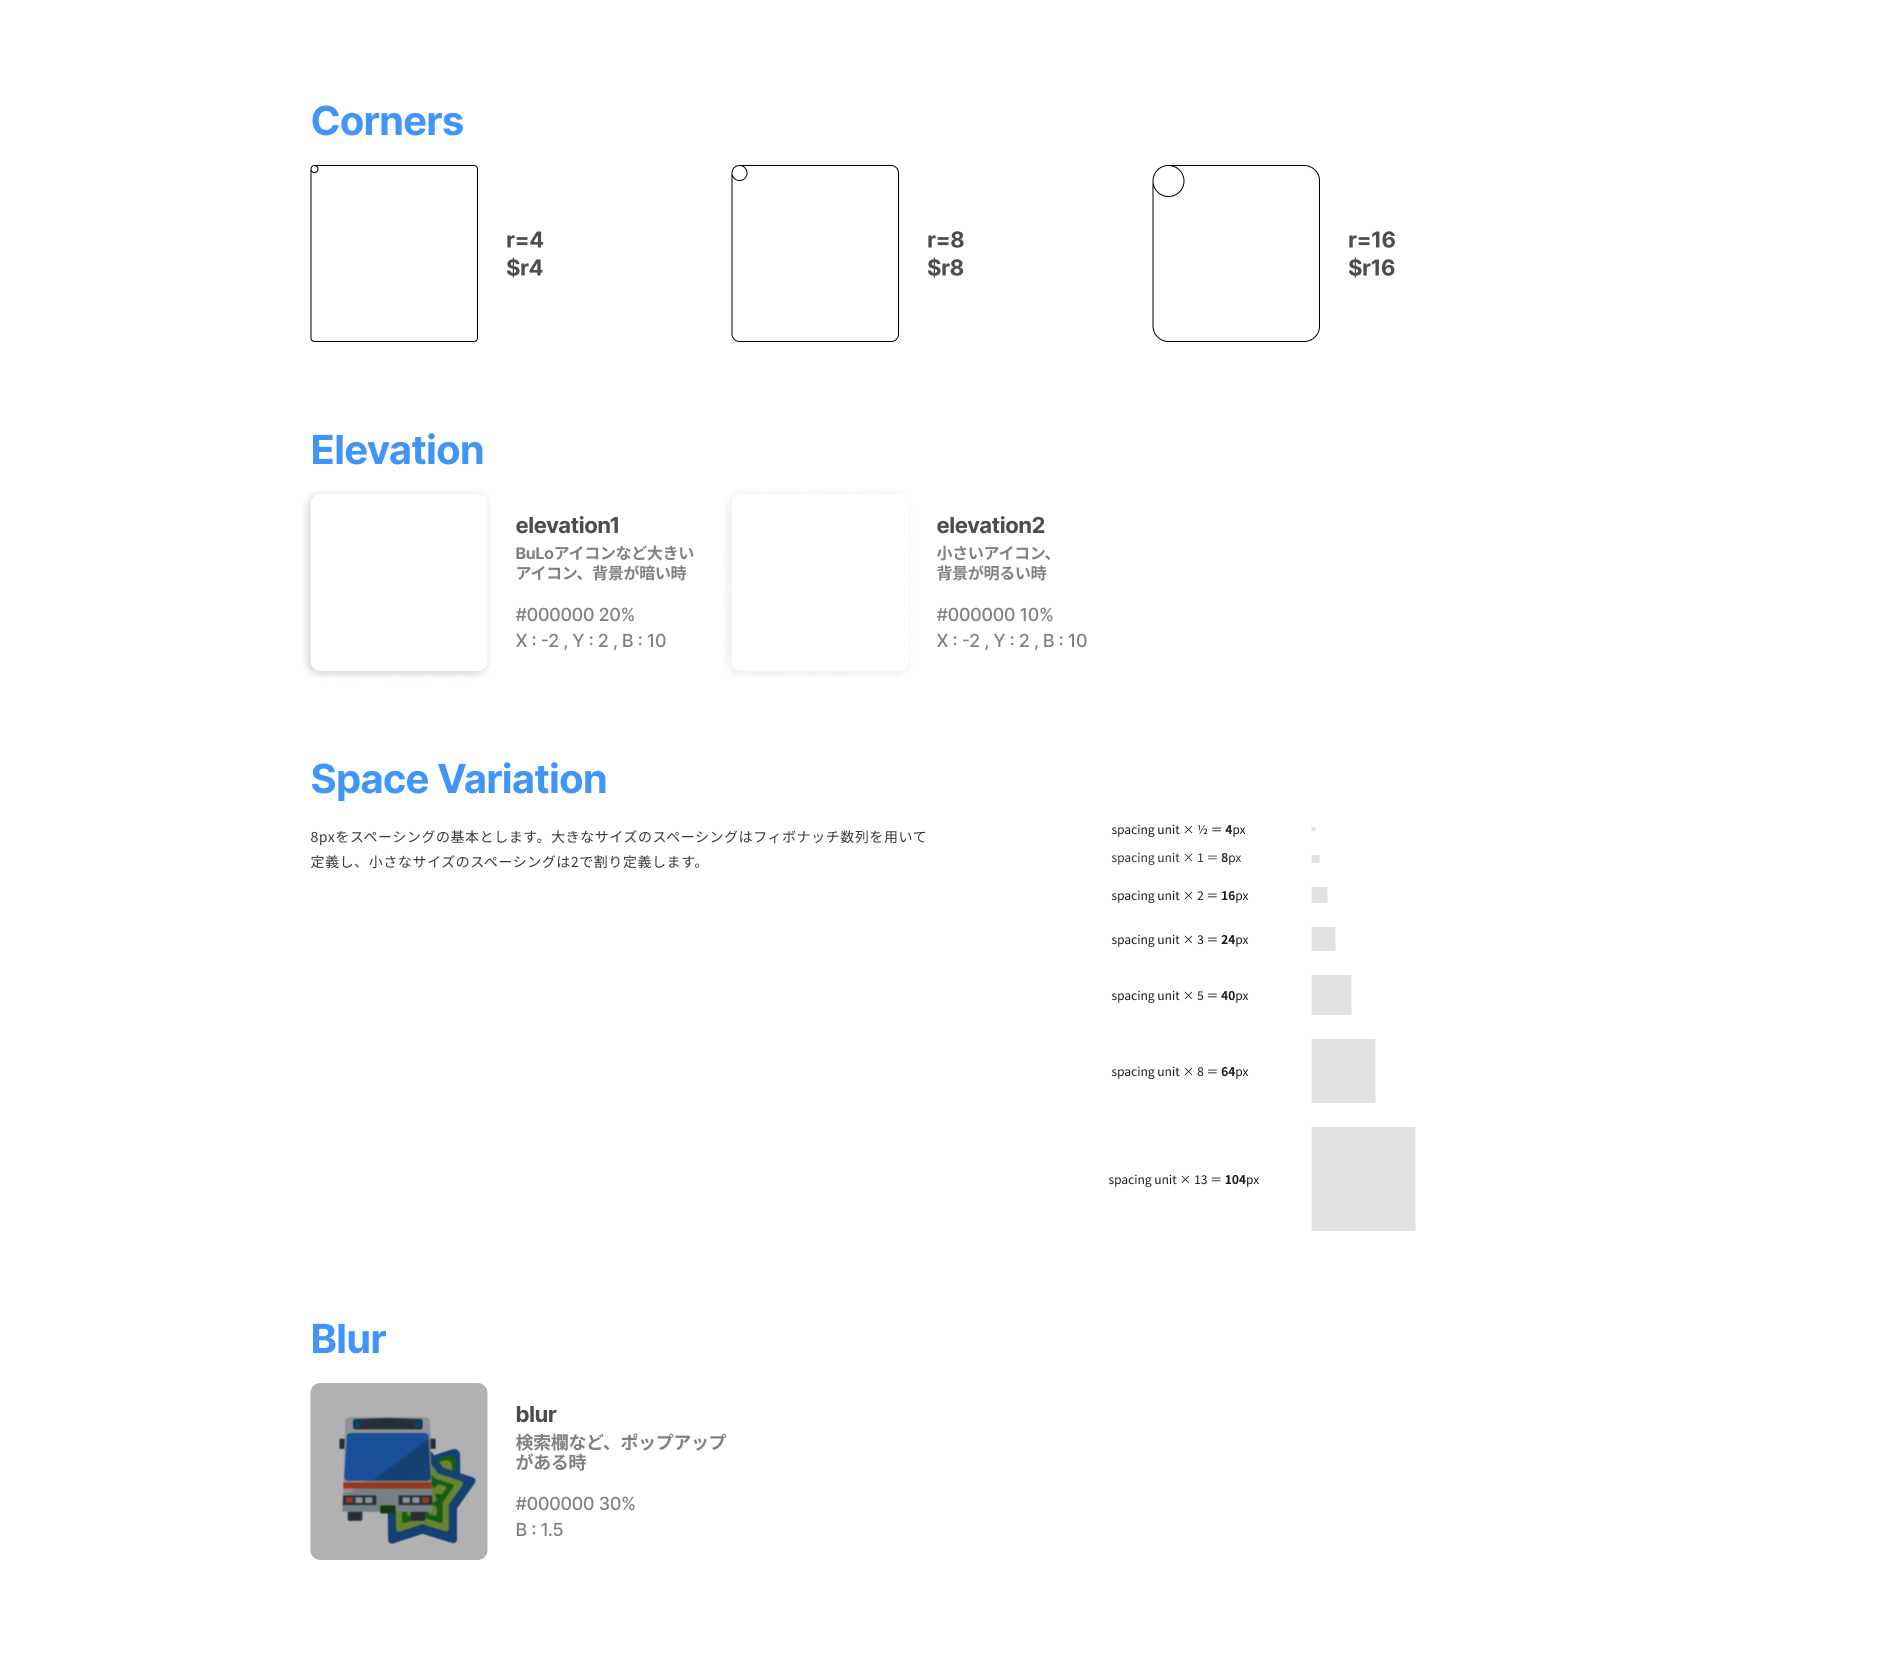
\includegraphics[width=10cm]{images/shapes.png}
    \caption{デザインシステム Shapes and Others}
    \label{fig:shapes}
\end{figure}
\bunseki{下村蒔里萌}

\section{システムの構成}
本サービスでは,マイクロサービスアーキテクチャを採用している.クライアントは,BFF (Backend for Frontend) を介して,バックエンドのマイクロサービスと通信する.
バックエンドのマイクロサービス間は,gRPCを用いて通信する.アーキテクチャ図を図\ref{fig:architecture}に示す.
\begin{figure}
    \centering
    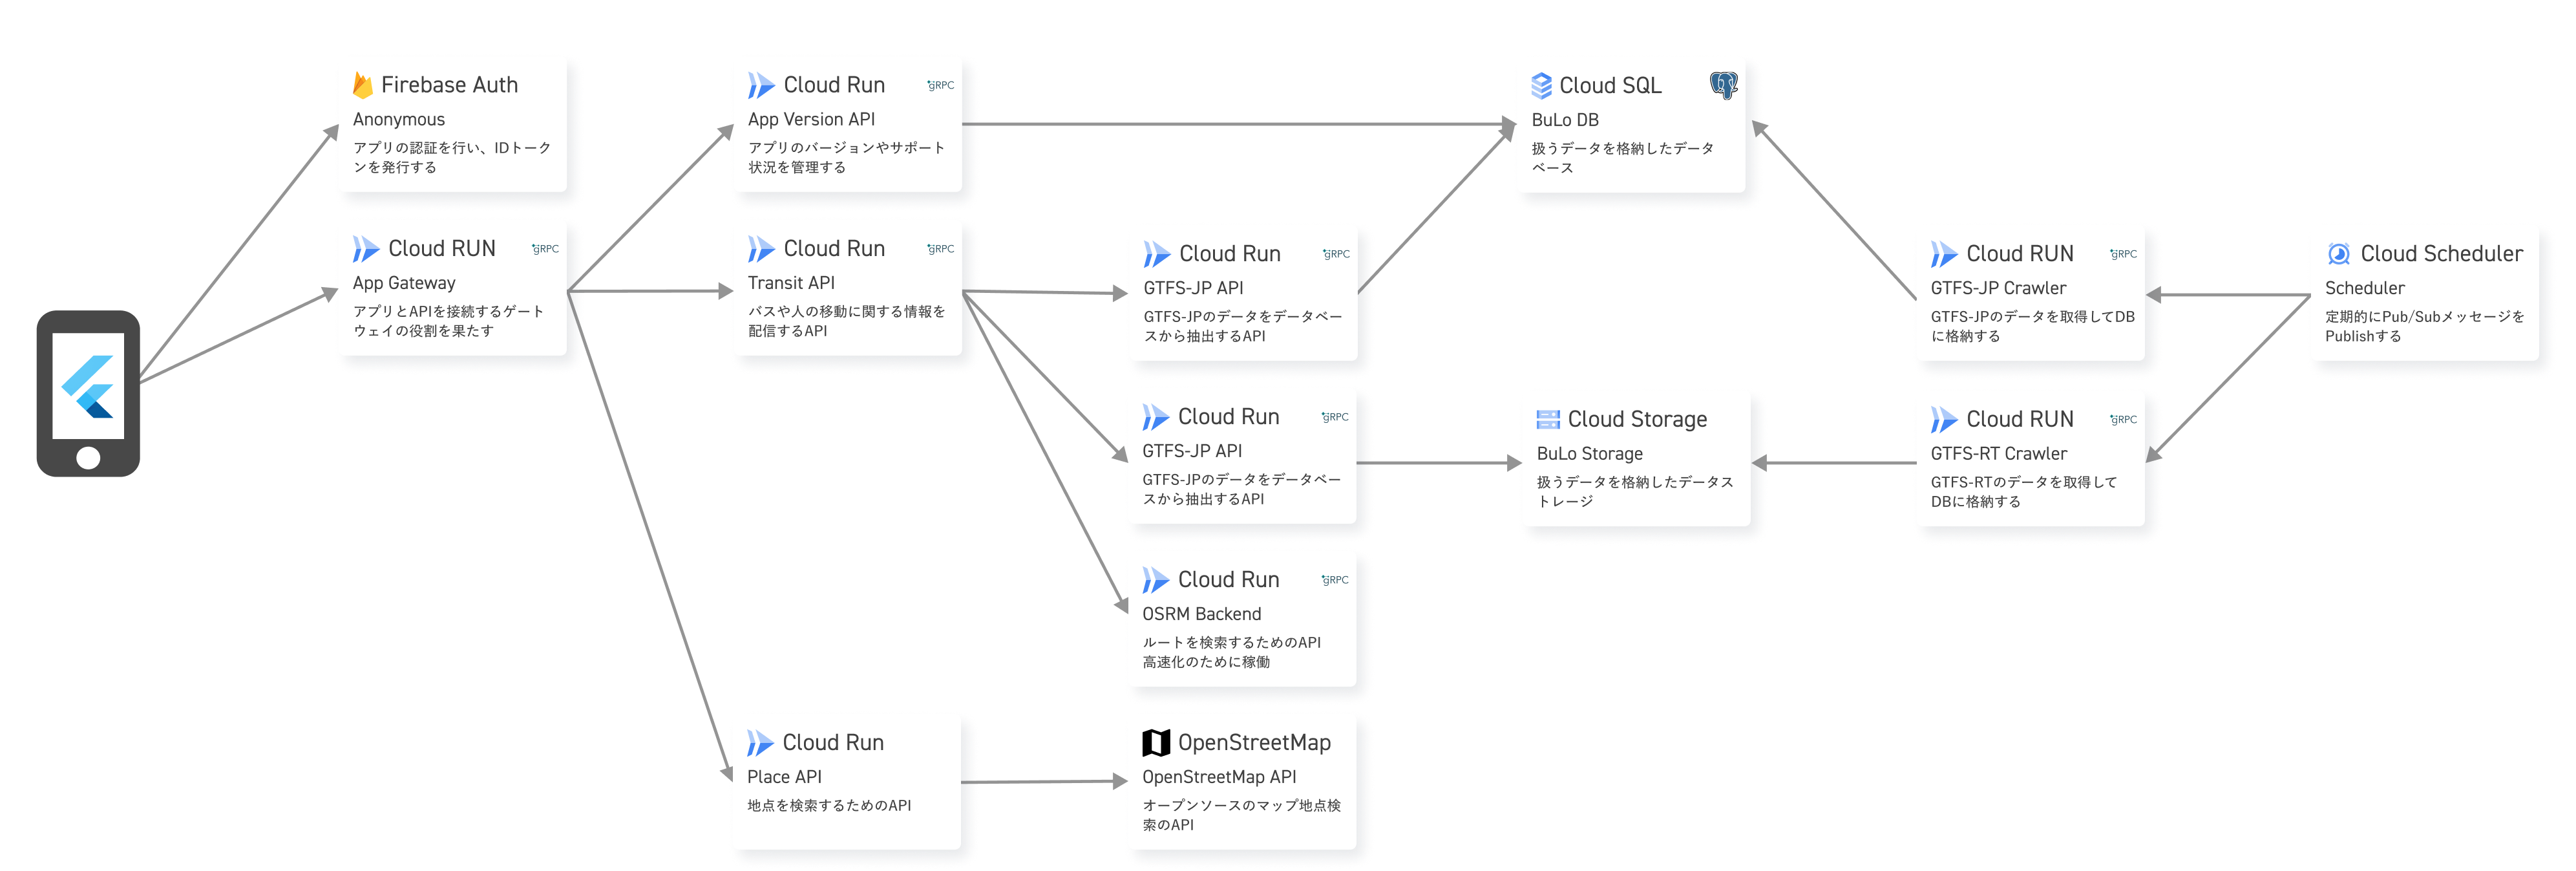
\includegraphics[width=14cm]{images/architecture_diagram.png}
    \caption{アーキテクチャ図}
    \label{fig:architecture}
\end{figure}
以下に,いくつかのマイクロサービスを抜粋して説明する.

\subsection{クライアントアプリケーション}
クライアントアプリケーションは,Flutter\footnote{https://flutter.dev/}を用いて開発した.Firebase Authentication\footnote{https://firebase.google.com/products/auth}を用いて,ユーザの匿名認証を行う.生成されたIDトークンを用いて,App Gatewayと通信をする.App Gatewayは,バックエンドのマイクロサービスと通信をして,クライアントが扱いやすい形で,データを返却する.高度なビジネスロジックをフロントエンド側で持たず,できる限りバックエンド側に切り出すようにした.

\subsection{Transit API}
本サービスで最も重要なマイクロサービスの一つである.クライアントアプリケーション内のTime-Distance ViewやRoute Viewを提供するために必要な情報を,GTFS-JPおよびGTFS-RTのデータから計算する.

\subsection{Place API}
地点を検索する際に,入力されたキーワードから,マッチする地点を検索するマイクロサービスである.検索には,OpenStreetMap\footnote{https://www.openstreetmap.org/}のデータからジオコーディングを行う,Nominatim\footnote{https://nominatim.org/}というオープンソースのジオコーディングツールを使用した.
\bunseki{及川寛太}

\section{使用した技術}
\subsection{Flutter}
当初は,iOSアプリをSwiftで,AndroidアプリをKotlinで開発する予定であったが,開発期間が短いことや人数が少ないことから,1つのコードベースで2つのプラットフォームをサポートできる,Flutterを採用した.

\subsection{GraphQL}
本サービスでは,当初,GraphQLサーバを介して,バックエンドのマイクロサービスと通信していた.
GraphQLのデメリットや,マイクロサービス間では,gRPCによる通信が行われていたことから,gRPCを用いて通信するように変更した.

\subsection{gRPC}
本サービスでは,マイクロサービス間通信,および,バックエンドのマイクロサービスとクライアント間通信にgRPCを用いている.

\subsection{PostgreSQL}
本サービスでは,GTFS-JPの静的データを保存し,各サービスからアクセスするために使用する.

\subsection{Google Cloud Platform}
本サービスの,データベースサーバはCloudSQL\footnote{https://cloud.google.com/sql/},バックエンドのマイクロサービスはCloud Run\footnote{https://cloud.google.com/run/}上で稼働している.
サーバレスサービスにより,サーバの管理にリソースを割くことなく,開発に集中することができる.
\bunseki{及川寛太}
% プロダクト
\include{process}% 活動
\chapter{今後の予定}
今後の予定は,1つ目に,複数事業者に対応させることを目指す.現状のバージョンでは函館バスのみしか対応していない.これを拡張し,函館市電やJR,また函館市以外のバス事業者にも対応させる.2つ目に乗り換えに対応させることを目指す.バスを利用する上で目的地まで行くのに乗り換えが起こることは多くある.また,すでに「乗り換えに対応して欲しい」という指摘が多く寄せられているので乗り換えに対応させることをを目指す.3つ目にパフォーマンスの向上を図る.現状のバージョンでは,住所を検索する際や,路線を検索する際,結果が出るまでに時間がかかってしまっている.本サービスは「ひとめぼれ」をコンセプトとしているため,このレスポンスの遅さを改善することを目指す.4つ目に,Route Viewでのルートの表示を目指す.ユーザのルートの表示の目処は立っている.しかし,函館バスが提供しているデータの中に,ルートの情報がないため,バスのルートの表示の目処が立っていない.そこでどのようにしてルートを表示するかを考え,実装を行う.最後に,調査に基づいてUI/UXの改善を行う.すでに中間発表会や成果発表会でUI/UXの改善点を指摘された.それらの指摘に加えて,一般リリースをしたあとの,ユーザのフィードバックをもとに改善を行い,より使いやすいアプリにしていく.
\bunseki{大津武琉}% ロードマップ
\chapter{学び}

\section{個人の学び}
\subsection{稲田敬介}
\bunseki{稲田敬介}

\subsection{及川寛太}
\bunseki{及川寛太}

\subsection{大津武琉}
\bunseki{大津武琉}

\subsection{下村蒔里萌}
\bunseki{下村蒔里萌}

% プロジェクトを通しての学び



% 以降、付録(付属資料)であることを示す
\begin{appendix}

\chapter{使用した技術・ツール・知識}

\section{フレームワーク}
\subsection{Flutter}
モバイルアプリのフレームワークとしてFlutter\footnote{https://flutter.dev/}を用いた.Android,iOSの両者にサービスを展開する上でKotlin,Swiftそれぞれでネイティブアプリを作成する事も検討したが,グループの規模とメンバーの技術力を考慮して,クロスプラットフォーム開発が可能であるFlutterを用いることに決定した.

\section{ツール}
\subsection{Discord}
本グループの主な連絡手段としてDiscord\footnote{https://discord.com/}を使用した.プロジェクトの連絡はもちろん,日常生活で起こったことなどをDiscordで共有することによりチームワークの向上を実現することができた.

\subsection{Notion}
本グループでは情報を管理するツールとしてNotion\footnote{https://www.notion.so/}を使用した.議事録,日報,週報,プロダクトバックログをそれぞれページにまとめることにより,情報を見やすくすることができた.今後も情報の管理ツールとして使用をしていく.

\subsection{GitHub}
GitHub\footnote{https://github.com/}とはソースコードのバージョン管理システムである.このツールを用いることでチームでのアプリ開発を効率的に行うことができる.本グループではフロントエンド,バックエンドでそれぞれリポジトリを作成し,アプリの開発を進めている.今後はより一層アプリの開発を進めることとなるため,GitHubを利用していく.
\pagebreak
\subsection{Figma}
Figma\footnote{https://www.figma.com/}とは,ホームページやアプリケーションなどのワイヤーフレームを作成できるツールである.中間発表スライドの作成,プロトタイプの作成,函館バス訪問の際に使用したスライドの作成に使用した.コンポーネントやレスポンシブを意識し,ワイヤーフレームを作成することで,今後の開発がスムーズになるようにした.

\subsection{Slack}
本プロジェクトの主な連絡手段としてSlack\footnote{https://slack.com/}を使用した.本グループでは主な連絡手段としてDiscordを利用していたが,プロジェクトではSlackを利用するとなったため使用した.細かくチャンネルを分けることで情報がどこにあるかをわかりやすくすることができた.また,メンションという機能を利用することにより教員,プロジェクトメンバー,TAとそれぞれに通知が行くようにすることで効率の良い意思疎通を行うことができた.

\subsection{Miro}
Miro\footnote{https://miro.com/}はオンラインでホワイトボードを利用できるツールである.ブレインストーミングなど,メンバーで一斉に意見を書くときに使用した.Miroを使用することにより,メンバーそれぞれの意見,考えを効率よく共有することができた.現在は同じような機能を持ったFigJamを利用している.

\subsection{FigJam}
FigJam\footnote{https://www.figma.com/}はオンラインでホワイトボードを利用できるツールである.Miroと同じようなツールだが本グループではFigmaを利用しており同じサービス元であるためFigJamへと移行した.

\subsection{Google Drive}
Google Drive\footnote{https://drive.google.com}とはGoogleが提供するオンラインストレージサービスである.これを用いることにより手軽にファイルの共有を行うことができる.また昨年度のファイル履歴を見返すこともでき,資料作り,プロジェクトの進め方の参考とした.
\pagebreak
\section{マネジメント}
\subsection{リスクマネジメント}
プロジェクトを行ううえでリスクは必ず存在する.リスクマネジメント\cite{risk}はそのリスクに対してどのように対策するのかを考える.まず初めにプロジェクトメンバーを3グループに分け,それぞれのチームでメンバーが持ち寄った起こりそうなリスクをまとめた.その後それぞれのリスクに対して,そのリスクが被る被害,発生確率,影響度,脅威,対策を考えた.脅威については発生確率,影響度を掛け合わせたものであり,脅威の値が大きいほど対策するべき優先度が高いものとなる.

\chapter{活用した講義}
\section{アジャイルワークショップ}
アジャイルコーチの永瀬氏に,本プロジェクトで用いるチーム開発の手法であるアジャイル開発について講義をしていただいた.まず,本ワークショップの前に事前知識を得るため,アジャイル開発についてのビデオを視聴した.その知識をもとに永瀬氏からアジャイル開発とはなにか,アジャイル開発で用いられるスクラムとはなにかを学んだ.また,最後に講義を受けているメンバーを5人ずつのチームにし,スクラムについてのクイズ大会を行った.これにより,楽しみながらスクラムについて学ぶことができ,スクラムについての共通認識を持つことができた.

\section{フィールドワーク講座}
本プロジェクトの担当教員でもある,南部美砂子准教授,元木環准教授に講義をしていただき,フィールドワークに関する基本的な考え方,ありがちな間違いをご教授いただいた.収束的なフィールドワークでは,思い込みや認識の狭さなどを超えられないため,フィールドワークには問題を探しにいくのではないこと,また,人々の行為や相互行為には必ず理由や動機が存在し,それらを理解することをフィールドワークの目的とすることを学んだ.

\bunseki{稲田敬介}

\chapter{夏季休暇中の活動}

\bunseki{稲田敬介}
\end{appendix}

%======================================================================
%\backmatter

% 参考文献
\begin{thebibliography}{9}
 \bibitem {ラベル} 著者名. 書籍名. 出版社,  年号.
 \bibitem {A2} ほげほげお. うんたらかんたら,  2003.
\end{thebibliography}

\end{document}
